% В этом шаблоне используется класс spbau-diploma. Его можно найти и, если требуется, 
% поправить в файле spbau-diploma.cls
\documentclass{spbau-diploma}
\usepackage{pdfpages}
\usepackage{subfiles}
\usepackage{listings}
\usepackage{xcolor}
\usepackage{minted}
\usepackage{caption}
\usepackage{hyperref}
\usepackage[noend]{algpseudocode}
\usepackage{algorithm}
\usepackage{amssymb}
\usepackage{amsmath}
\usepackage[stable]{footmisc}
\usepackage{subcaption}
\usepackage{changepage}
\begin{document}
\renewcommand\listingscaption{Листинг}
\newenvironment{megaalgorithm}[1][htb]{
    \floatname{algorithm}{Стратегия}%% Update algorithm name
   \begin{algorithm}[H]
  }{\end{algorithm}}

%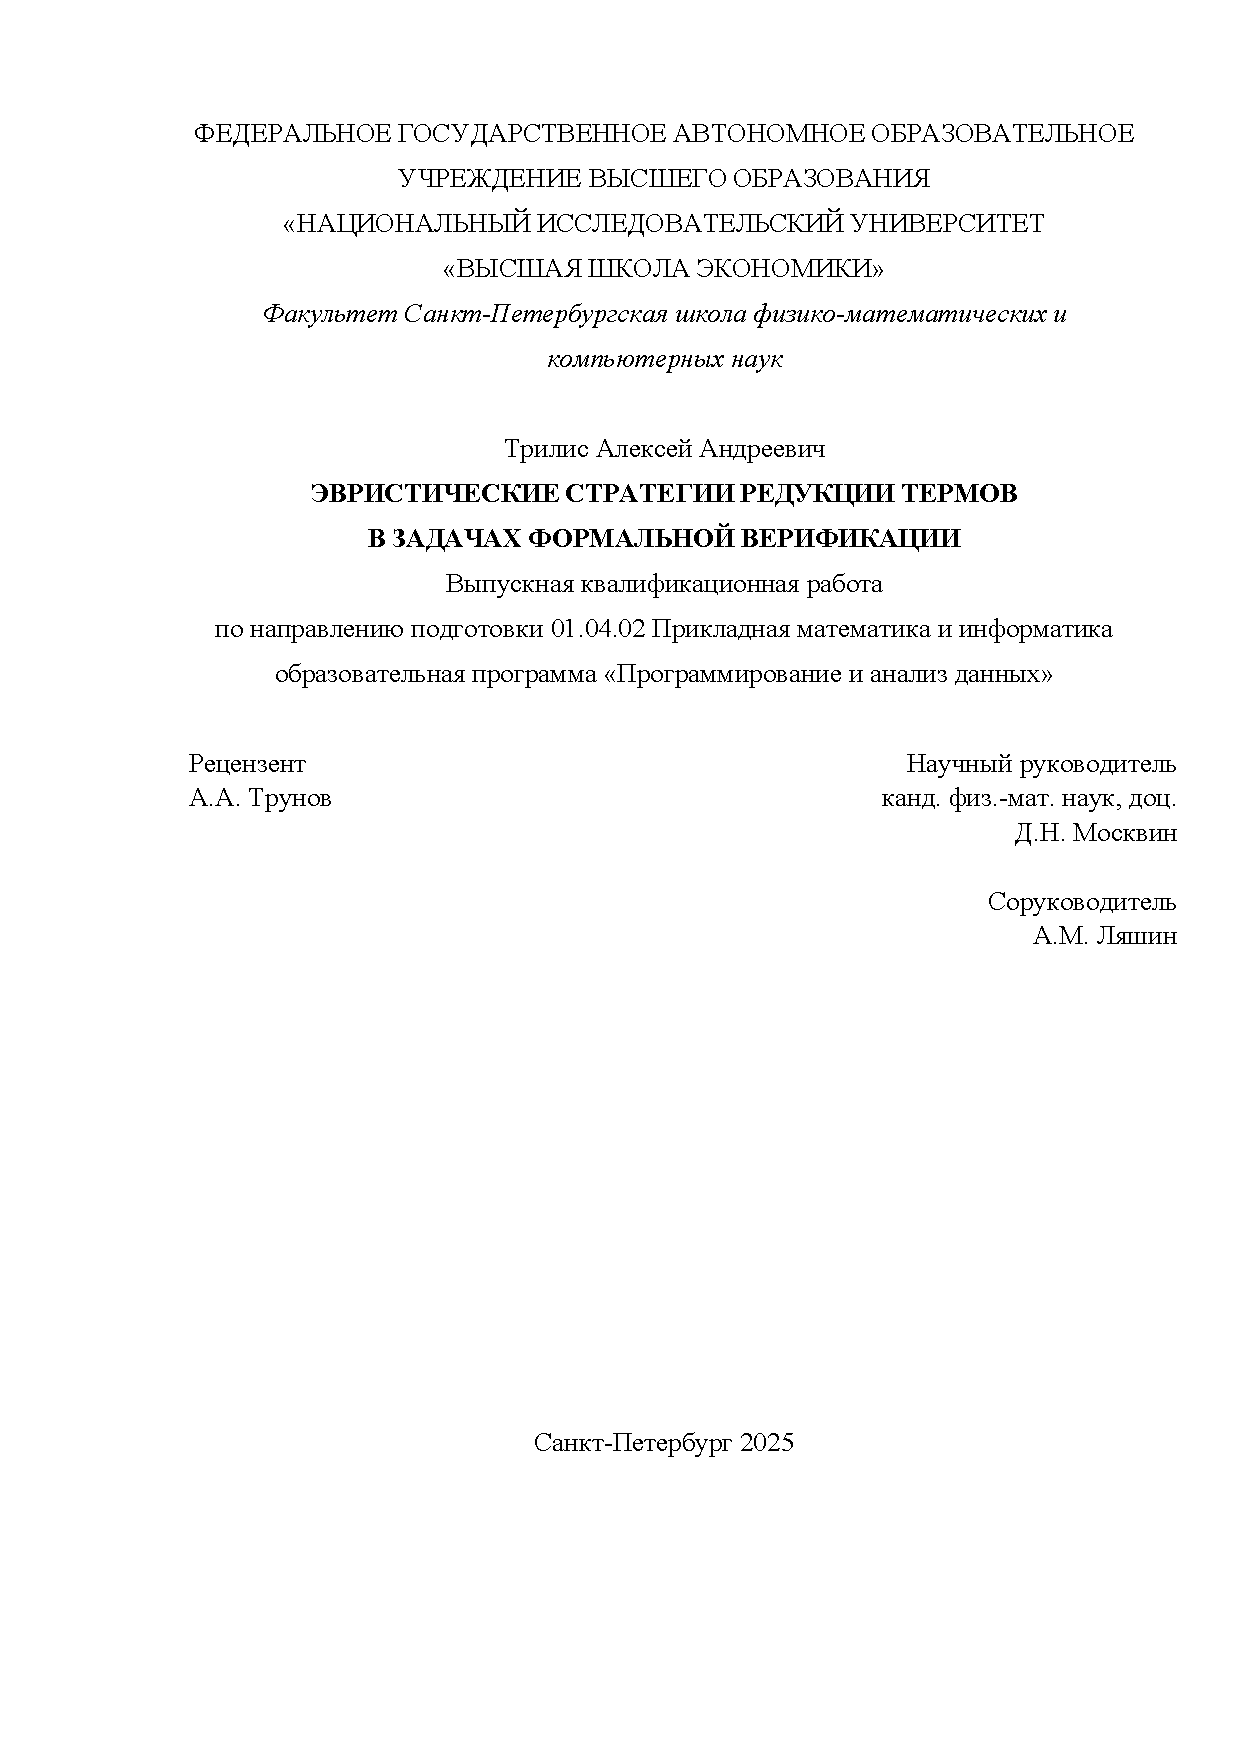
\includepdf[pages=-]{title.pdf}
\maketitle
{
\large \centering
\textbf{Эвристические стратегии редукции термов\\в задачах формальной верификации}
\bigskip
\bigskip

Магистерская диссертация
\bigskip
\bigskip

Трилис Алексей Андреевич
\bigskip
\bigskip

Руководитель: Ляшин Андрей Михайлович
\bigskip
\bigskip

Рецензент: Трунов Антон Александрович
\bigskip
\bigskip

НИУ ВШЭ --- Санкт-Петербург
\bigskip
\bigskip

2025

}
\tableofcontents


\section*{Аннотация}
\subfile{sections/abstract}

\section*{Введение}
\subfile{sections/introduction}

\section{Обзор предметной области}
\subfile{sections/1}

\section{Разработка стратегий}
\subfile{sections/2}

\section{Сравнение стратегий}
\subfile{sections/3}

\section*{Заключение}
\subfile{sections/conclusion}


\bibliographystyle{ugost2008my}
\bibliography{diploma.bib}
\end{document}
